\documentclass[../main.tex, class=article, 12pt]{subfiles}
\usepackage{float}
\usepackage{amsthm}
\usepackage{amsmath}
\usepackage{amssymb}
\usepackage{hyperref}
\usepackage{caption}
\usepackage{mathtools}
\usepackage{graphicx}
\usepackage{todonotes}
\usepackage{tcolorbox}
\graphicspath{{./images}}




\begin{document}

\begin{definition}
        Sia $ f : A \to \mathbb{R} $ una fuzione
        \begin{itemize}
                \item $ f $ si dice superiormente limitata su $ A $ se $ \exists M > 0 $ tale che $ f(x) \le M $ per ogni $ x \in A $.
                \item $ f $ si dice inferiormente limitata su $ A $ se $ \exists M : f(x) \ge -M  $ per ogni $ x \in A $.
                \item $ x_m \in A $ si dice punto di massimo di $ f $ in $ A $ se $ f(x) \le f(x_m) \forall x \in A $.
                \item $ x_m \in A $ si dice punto di minimo di $ f $ in $ A $ se $ f(x_m) \le f(x)  $ per ogni $ x \in A $.
                \item $ M \in \mathbb{R} $ è detto estremo superiore di $ f $ in $ A $ se:
        \end{itemize}
        \todo{LEZ 8/4: :Aggiungere sottoliste}

        \begin{figure}[H]
          	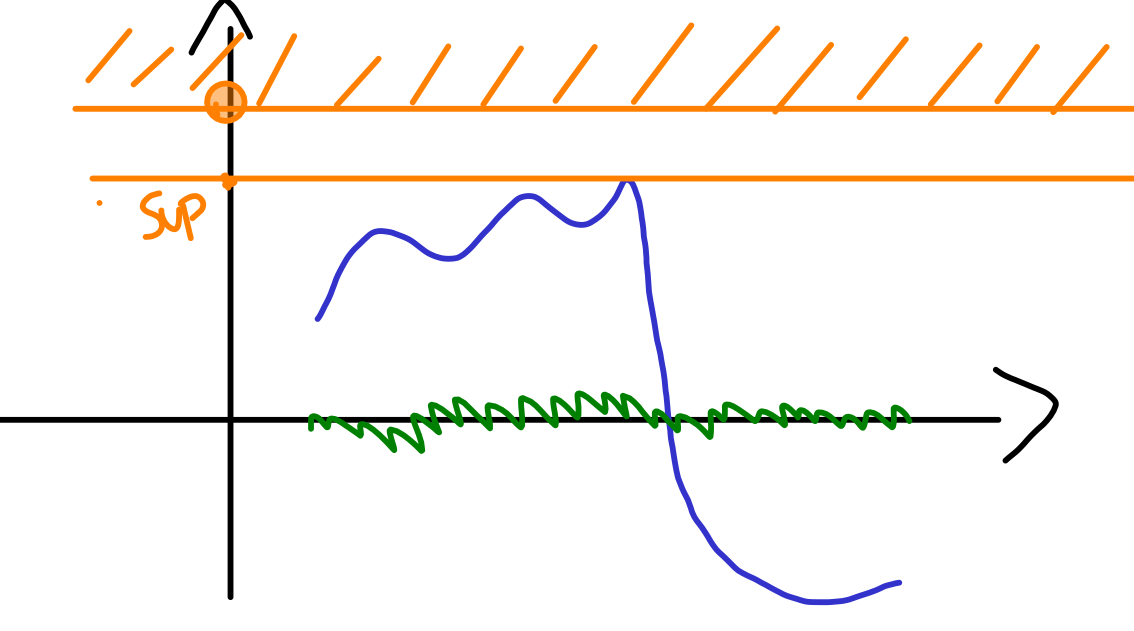
\includegraphics[width=\linewidth]{grafico_massimo_superiore.png}
          	\caption{}
                \label{fig:grafico_massimo_superiore.png}
        \end{figure}
        \begin{figure}[H]
          	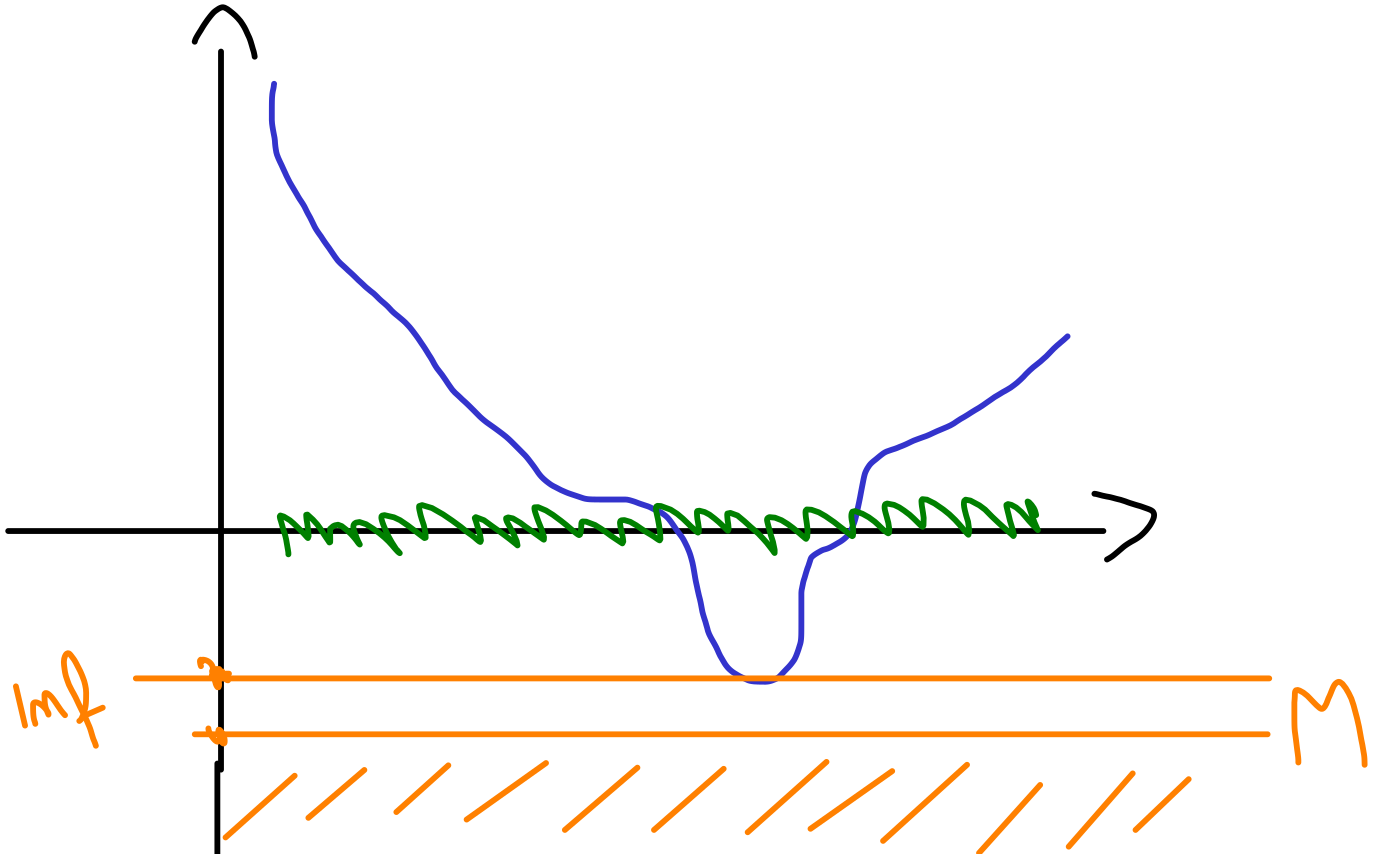
\includegraphics[width=\linewidth]{grafico_minimo_inferiore.png}
          	\caption{}
                \label{fig:grafico_minimo_inferiore.png}
        \end{figure}
\end{definition}

\newpage
Una funzione si dice realizzare il massimo se $ \exists x_m $ punto di massimo. In questo caso si dice $ sup(f) = max(f) $. \par
Una funzione si dice realizzare il minimo se $ \exists x_m $ punto di massimo. In questo caso si dice $ inf(f) = min(f) $.

\begin{tcolorbox}
\begin{theorem}
        Supponiamo $ f $ sia superiormente limitata, allora $ \exists \sup(f)  \in \mathbb{R}$.
\end{theorem}
\begin{theorem}
        Supponiamo $ f $ sia inferiormente limitata, allora $ \exists \inf(f)  \in \mathbb{R}$
\end{theorem}
\end{tcolorbox}
\todo{LEZ 8/4: dividere il testo in due sezioni}


\newpage
\subsection{Teorema di Weierstrass}\label{sec:teorema_di}
\begin{tcolorbox}
        \begin{theorem}
                Sia $ f : [a,b] \to \mathbb{R} $  una funzione \underline{continua}, allora $ \exists x_M, x_m$ rispettivamente punto di massimo e punto di minimo, in particolare $ f $ realizza il massimo e il minimo.
        \end{theorem}
\end{tcolorbox}

\begin{tcolorbox}
       \begin{theorem}
               Sia $ f : [a,b] \to \mathbb{R} $ una funzione \underline{continua}, sia $ f(x) \le c \le f(b) $, allora $ \exists x \in [a, b) $ tale che $ f(x) = c $.
        
       \end{theorem} 
\end{tcolorbox}
        \begin{figure}[h]
          	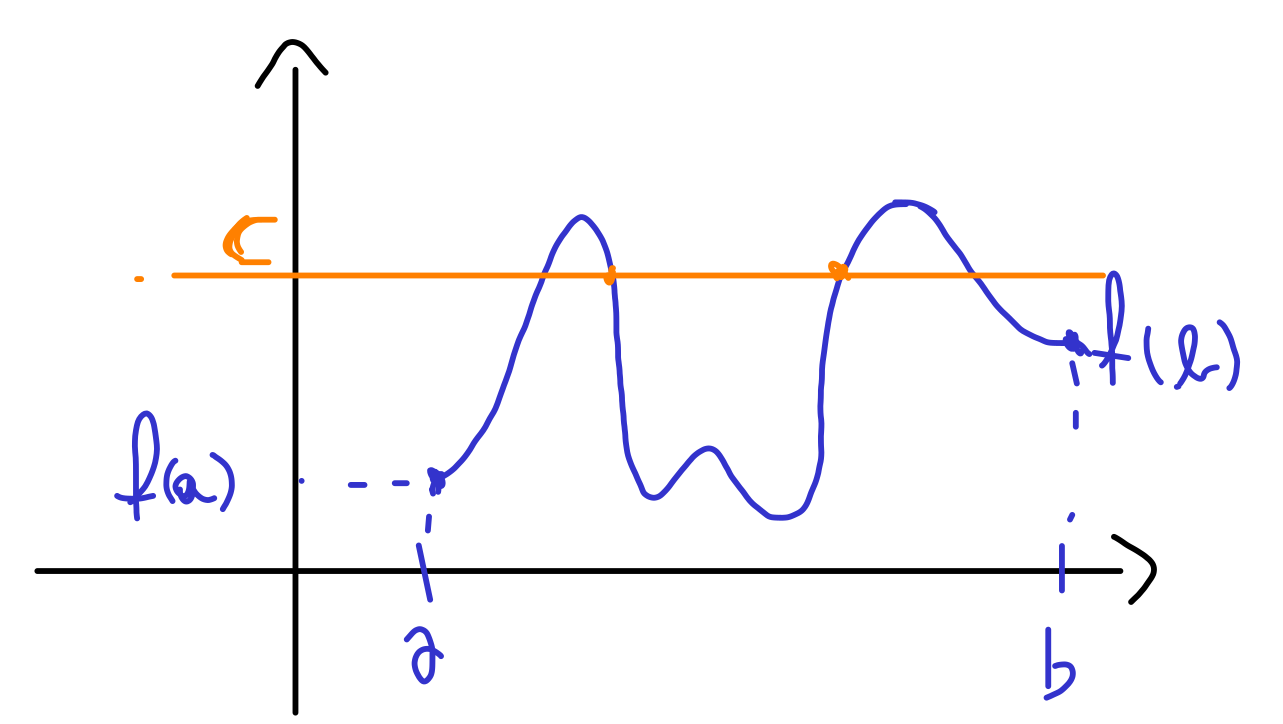
\includegraphics[width=\linewidth]{grafico_teorema_valore_medio.png}
          	\caption{}
                \label{fig:grafico_teorema_valore_medio.png}
        \end{figure}

\begin{tcolorbox}
        \begin{corollario}
                \textbf{(Weierstrass + valore medio)} Se $ f : [a, b] \to \mathbb{R} $ è una funzione continua allora $ InF = [\inf(f), \sup(f)] $, inoltre $ \inf(f) = \min(f) \in \mathbb{R} \quad  \sup(f) = \max(f) \in \mathbb{R}$
        \end{corollario}
\end{tcolorbox}








\end{document}
